\documentclass{article}

\usepackage{amsmath}
\usepackage{amsfonts}
\usepackage{graphicx}

\newcommand{\rr}{\mathbf{r}}
\DeclareMathOperator{\curl}{curl}

\begin{document}

{\bf Quiz \#13; Tuesday, date: 04/24/2018}

{\bf MATH 53 Multivariable Calculus with Stankova}

{\bf Section \#114; time: 2 -- 3:30 pm}

{\bf GSI name: Kenneth Hung}

{\bf Student name:}

\vspace*{0.25in}

\begin{enumerate}
\item Is there a vector field $\mathbf{G}$ on $\mathbb{R}^3$ such that $\curl \mathbf{G} = \langle \cos x, \sin y, z \rangle$? Explain.

\item {\em True / False?} Given a vector field $\mathbf{F} = \langle P, Q \rangle$ with $\frac{\partial Q}{\partial x} = \frac{\partial P}{\partial y}$ over the region given below.
\begin{center}
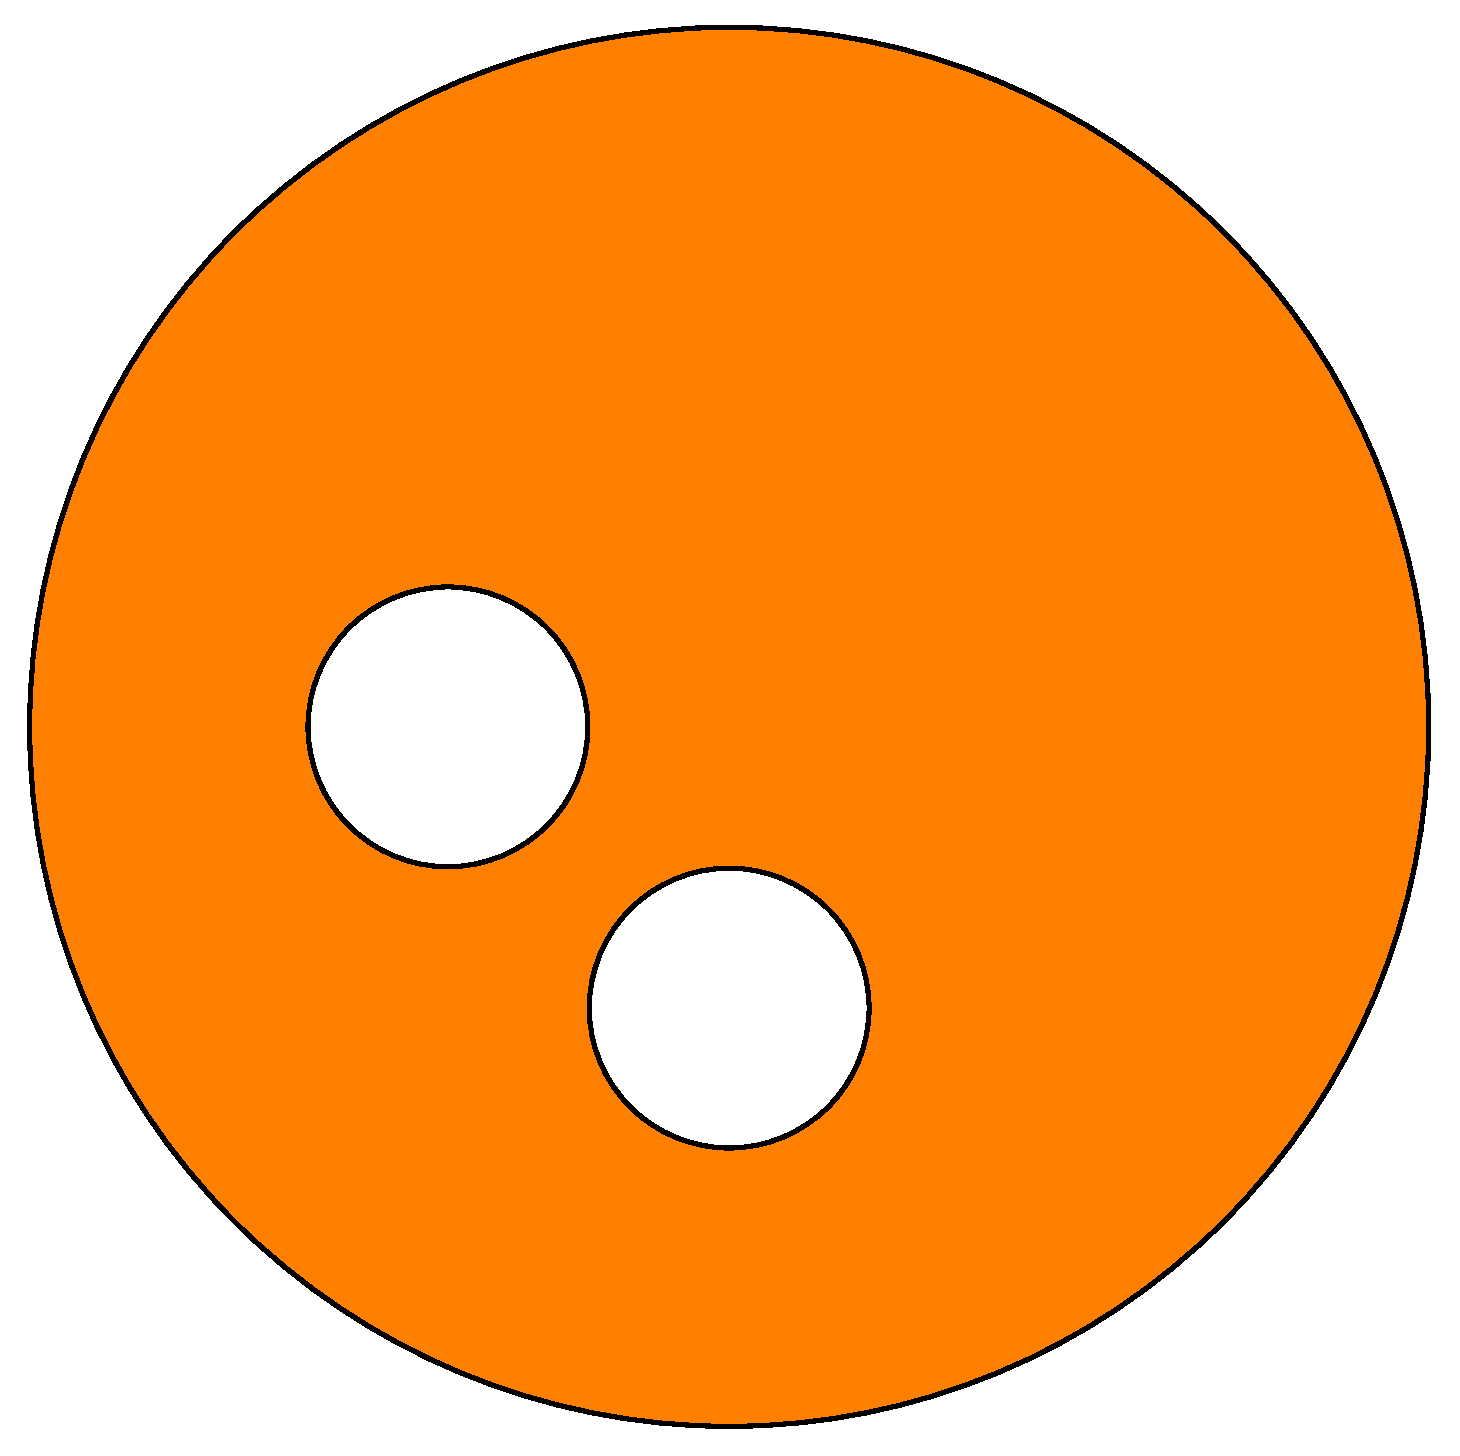
\includegraphics[width=0.4\textwidth]{quiz13dis114pic}
\end{center}
Suppose the big circle is $C_1$ and the small circles are $C_2$ and $C_3$, all counterclockwise, then
\[
\int_{C_1} \mathbf{F} \cdot d\rr = \int_{C_2} \mathbf{F} \cdot d\rr + \int_{C_3} \mathbf{F} \cdot d\rr.
\]

\item {\em True / False?} Surface of revolution of a positive differentiable function is always smooth.
\end{enumerate}

\end{document}